% !TEX program = xelatex
\documentclass[11pt,a4paper]{article}

\usepackage[margin=1.8cm]{geometry}
\usepackage{fontspec}
\usepackage{xcolor}
\usepackage{graphicx}
\usepackage{tikz}
\usepackage{enumitem}
\usepackage{tabularx}
\usepackage{booktabs}
\usepackage{hyperref}
\usepackage{microtype}

\definecolor{ink}{HTML}{1A1A1A}
\definecolor{mute}{HTML}{5C5C5C}
\definecolor{line}{HTML}{E6E6E6}
\definecolor{paper}{HTML}{FAFAFA}
\definecolor{chiiko}{HTML}{111111}

\setmainfont{TeX Gyre Pagella}
\setsansfont{Montserrat}

\newfontfamily\fPagella{TeX Gyre Pagella}
\newfontfamily\fTermes{TeX Gyre Termes}
\newfontfamily\fSchola{TeX Gyre Schola}
\newfontfamily\fBonum{TeX Gyre Bonum}
\newfontfamily\fChorus{TeX Gyre Chorus}
\newfontfamily\fAdventor{TeX Gyre Adventor}
\newfontfamily\fHeros{TeX Gyre Heros}
\newfontfamily\fMontserrat{Montserrat Light}
\newfontfamily\fMontserratMed{Montserrat Medium}
\newfontfamily\fRedHat{Red Hat Display Light}
\newfontfamily\fRedHatText{Red Hat Text}
\newfontfamily\fLMRoman{Latin Modern Roman}
\newfontfamily\fLiberation{Liberation Serif}
\newfontfamily\fBookman{URW Bookman}
\newfontfamily\fGothic{URW Gothic}
\newfontfamily\fCarlito{Carlito}
\newfontfamily\fDejaVu{DejaVu Sans}

\newcommand{\chiikologo}{%
  
\includegraphics[height=1.35cm]{../../public/chiikologosophie.png}%
}

\newcommand{\docheader}[1]{%
  \noindent
  \begin{tikzpicture}
    \fill[paper] (0,0) rectangle (\textwidth,2.1);
    \node[anchor=west] at (0.2,1.05) {\chiikologo};
    \node[anchor=east, align=right, text=ink] at (\textwidth-0.2,1.35) {%
      {\sffamily\bfseries\large Sophie Gomez --- Propuestas}\\[2pt]
      {\sffamily\color{mute}\small #1}\\[1pt]
      {\sffamily\color{mute}\footnotesize Chiiko · Documento de selección}
    };
  \end{tikzpicture}
  \vspace{0.35cm}
  {\color{line}\hrule height 0.6pt}
  \vspace{0.55cm}
}

\newcommand{\fontcard}[5]{%
  % #1 family cmd, #2 name, #3 vibe, #4 best use, #5 sample note
  \noindent
  \begin{tikzpicture}
    \draw[line, line width=0.7pt, fill=white] (0,0) rectangle (\textwidth,4.55);
    \node[anchor=north west, text=mute, font=\sffamily\footnotesize\bfseries] at (0.35,4.35) {PROPUESTA};
    \node[anchor=north east, text=mute, font=\sffamily\footnotesize, align=right] at (\textwidth-0.35,4.35) {#3};
    \node[anchor=north west, text=ink] at (0.35,3.9) {{\Large\bfseries\sffamily #2}};
    \node[anchor=north west, text=ink, font=#1] at (0.35,3.25) {%
      \fontsize{28}{32}\selectfont SOPHIE GOMEZ%
    };
    \node[anchor=north west, text=ink, font=#1] at (0.35,2.35) {%
      \fontsize{13}{17}\selectfont Actrice · Modèle · Silver Présence%
    };
    \node[anchor=north west, text=mute, font=#1, text width=\textwidth-0.8cm] at (0.35,1.75) {%
      \fontsize{10.5}{14}\selectfont
      Du théâtre au cinéma d'auteur, Sophie Gomez construit des personnages
      habités entre Mexico et l'Europe. Une présence précise, lumineuse, mémorable.%
    };
    \node[anchor=south west, text=mute, font=\sffamily\scriptsize] at (0.35,0.25) {Uso ideal: #4};
    \node[anchor=south east, text=mute, font=\sffamily\scriptsize] at (\textwidth-0.35,0.25) {#5};
  \end{tikzpicture}
  \vspace{0.35cm}
}

\pagestyle{empty}
\setlength{\parindent}{0pt}

\begin{document}
\color{ink}

\docheader{01 · Tipografías elegantes}

{\sffamily
\textbf{Instrucciones para Sophie}\\[4pt]
{\color{mute}
Este documento muestra \textbf{varias propuestas tipográficas} para el sitio.
Cada tarjeta usa la misma frase de marca para comparar con facilidad.
Marca 1--2 favoritas (titulares) y, si quieres, otra para cuerpo de texto.
}
}

\vspace{0.45cm}

\section*{{\sffamily 1. Serif clásicas / editoriales}}

\fontcard{\fPagella}{TeX Gyre Pagella (estilo Palatino)}{Elegante · cálida · editorial}{Titulares + bio}{Sensación premium sin ser rígida}

\fontcard{\fTermes}{TeX Gyre Termes (estilo Times)}{Clásica · prensa · legible}{Cuerpo de texto / press kit}{Tradicional, muy legible en párrafos}

\fontcard{\fSchola}{TeX Gyre Schola (estilo Schoolbook)}{Literaria · clara · sofisticada}{Bios largas y press kit}{Más abierta, fácil de leer}

\fontcard{\fBonum}{TeX Gyre Bonum (estilo Bookman)}{Amplia · editorial · amable}{Titulares medianos + texto}{Presencia suave, menos ``lujo duro''}

\fontcard{\fLMRoman}{Latin Modern Roman}{Académica · clara · clásica}{Bios y press kit}{Heredera de Computer Modern; muy legible}

\fontcard{\fLiberation}{Liberation Serif}{Sobria · profesional · casting}{CV / datos técnicos}{Tono casting / ficha técnica}

\fontcard{\fBookman}{URW Bookman}{Cálida · revista · fashion-lite}{Landing y modelo}{Cercana a look magazine}

\newpage
\docheader{01 · Tipografías elegantes (cont.)}

\section*{{\sffamily 2. Display / alto contraste (para el nombre)}}

\fontcard{\fChorus}{TeX Gyre Chorus}{Expresiva · firma · detalle}{Solo acentos o citas (no menú)}{Más personal; usar con moderación}

\noindent
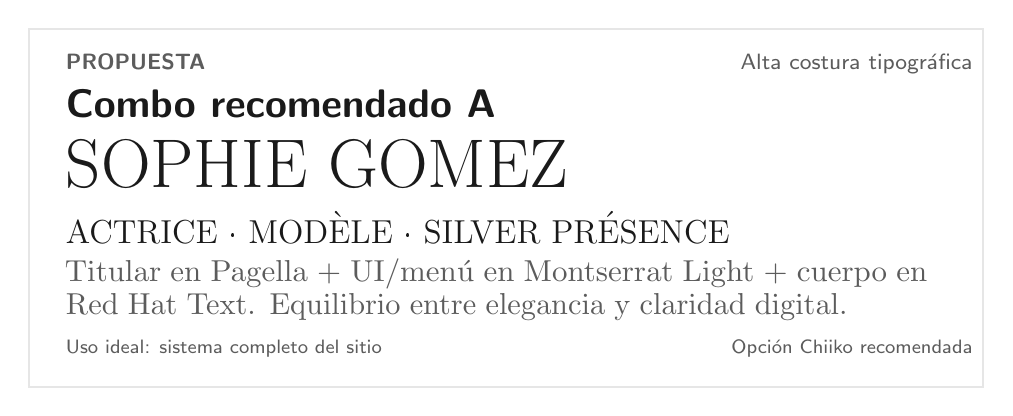
\begin{tikzpicture}
  \draw[line, line width=0.7pt, fill=white] (0,0) rectangle (\textwidth,4.55);
  \node[anchor=north west, text=mute, font=\sffamily\footnotesize\bfseries] at (0.35,4.35) {PROPUESTA};
  \node[anchor=north east, text=mute, font=\sffamily\footnotesize, align=right] at (\textwidth-0.35,4.35) {Alta costura tipográfica};
  \node[anchor=north west, text=ink] at (0.35,3.9) {{\Large\bfseries\sffamily Combo recomendado A}};
  \node[anchor=north west, text=ink, font=\fPagella] at (0.35,3.25) {%
    \fontsize{28}{32}\selectfont SOPHIE GOMEZ%
  };
  \node[anchor=north west, text=ink, font=\fMontserrat] at (0.35,2.35) {%
    \fontsize{12}{16}\selectfont ACTRICE · MODÈLE · SILVER PRÉSENCE%
  };
  \node[anchor=north west, text=mute, font=\fRedHatText, text width=\textwidth-0.8cm] at (0.35,1.75) {%
    \fontsize{10.5}{14}\selectfont
    Titular en Pagella + UI/menú en Montserrat Light + cuerpo en Red Hat Text.
    Equilibrio entre elegancia y claridad digital.%
  };
  \node[anchor=south west, text=mute, font=\sffamily\scriptsize] at (0.35,0.25) {Uso ideal: sistema completo del sitio};
  \node[anchor=south east, text=mute, font=\sffamily\scriptsize] at (\textwidth-0.35,0.25) {Opción Chiiko recomendada};
\end{tikzpicture}
\vspace{0.35cm}

\section*{{\sffamily 3. Sans elegantes (menú, UI, CTAs)}}

\fontcard{\fMontserrat}{Montserrat Light / SemiBold}{Moderna · moda · limpia}{Menú, botones, labels}{Muy usada en portfolios fashion}

\fontcard{\fMontserratMed}{Montserrat Medium}{Firme · contemporánea · marca}{Nombre en nav + CTAs}{Un poco más ``sólida'' que Light}

\fontcard{\fRedHat}{Red Hat Display Light}{Tech-editorial · clara · actual}{Hero keywords + UI}{Elegante sin parecer ``startup purple''}

\fontcard{\fRedHatText}{Red Hat Text}{Legible · profesional · web}{Párrafos y contacto}{Excelente lectura en pantalla}

\fontcard{\fAdventor}{TeX Gyre Adventor}{Geométrica · gallery · bold presence}{Títulos de sección}{Más carácter; menos neutra}

\fontcard{\fHeros}{TeX Gyre Heros (estilo Helvetica)}{Minimal suizo · casting}{UI completa}{Clásico de diseño suizo/minimal}

\fontcard{\fGothic}{URW Gothic}{Editorial soft · contemporánea}{Menú + footer}{Sans con personalidad suave}

\fontcard{\fCarlito}{Carlito}{Humana · limpia · accesible}{Formularios / datos}{Muy legible en móviles}

\newpage
\docheader{01 · Tipografías elegantes (cont.)}

\section*{{\sffamily 4. Combinaciones listas para elegir}}

\renewcommand{\arraystretch}{1.45}
{\sffamily\small
\begin{tabularx}{\textwidth}{@{}>{\bfseries}p{2.1cm} X X p{2.6cm}@{}}
\toprule
Código & Titulares & Cuerpo / UI & Sensación \\
\midrule
A & Pagella & Montserrat + Red Hat Text & Editorial premium \\
B & Termes & Heros & Casting / cine sobrio \\
C & Schola & Montserrat Light & Literaria + moda \\
D & Bookman & Red Hat Display & Fashion magazine \\
E & Latin Modern Roman & Carlito & Clara / académica \\
F & Adventor & Heros & Gallery contemporánea \\
G & Pagella & Gothic & Soft luxury \\
H & Chorus (solo firma) + Pagella & Montserrat & Detalle artístico \\
\bottomrule
\end{tabularx}
}

\vspace{0.7cm}
\section*{{\sffamily 5. Cómo marcar tu elección}}

{\sffamily\color{mute}
\begin{enumerate}[leftmargin=1.2em,itemsep=0.25em]
  \item Elige \textbf{una tipografía (o combo)} para el nombre ``SOPHIE GOMEZ''.
  \item Elige \textbf{una sans} para menú, botones e idiomas (FR / ES / EN).
  \item Si quieres, elige otra para bios largas (o usa la misma del combo).
  \item Anota aquí tu preferencia:
\end{enumerate}
}

\vspace{0.4cm}
\noindent
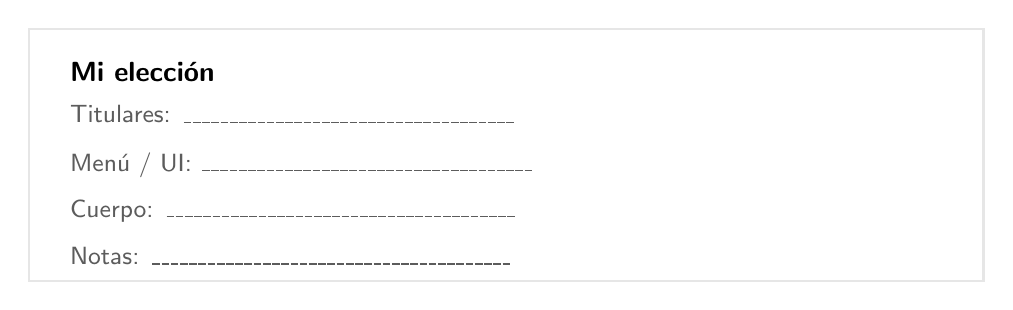
\begin{tikzpicture}
  \draw[line, line width=0.8pt] (0,0) rectangle (\textwidth,3.2);
  \node[anchor=north west, font=\sffamily\bfseries] at (0.4,2.9) {Mi elección};
  \node[anchor=north west, font=\sffamily\small, text=mute] at (0.4,2.35) {Titulares: \_\_\_\_\_\_\_\_\_\_\_\_\_\_\_\_\_\_\_\_\_\_\_\_\_\_\_\_\_\_\_\_\_\_\_\_};
  \node[anchor=north west, font=\sffamily\small, text=mute] at (0.4,1.75) {Menú / UI: \_\_\_\_\_\_\_\_\_\_\_\_\_\_\_\_\_\_\_\_\_\_\_\_\_\_\_\_\_\_\_\_\_\_\_\_};
  \node[anchor=north west, font=\sffamily\small, text=mute] at (0.4,1.15) {Cuerpo: \_\_\_\_\_\_\_\_\_\_\_\_\_\_\_\_\_\_\_\_\_\_\_\_\_\_\_\_\_\_\_\_\_\_\_\_\_\_};
  \node[anchor=north west, font=\sffamily\small, text=mute] at (0.4,0.55) {Notas: \_\_\_\_\_\_\_\_\_\_\_\_\_\_\_\_\_\_\_\_\_\_\_\_\_\_\_\_\_\_\_\_\_\_\_\_\_\_\_};
\end{tikzpicture}

\vspace{0.8cm}
{\sffamily\color{mute}\footnotesize
Chiiko · Propuesta tipográfica para Sophie Gomez · Documento interno de selección
}

\end{document}
